\documentclass[11pt]{article}

\usepackage{float}
\usepackage{hyperref}
\usepackage{graphicx}
% formatting
\usepackage{fullpage}
\usepackage{verbatim}
\usepackage{moreverb}
\usepackage{minted}
\usepackage{parskip}
\usepackage{hyperref}
\usepackage{microtype}
\usepackage{appendix}
\let\verbatiminput=\verbatimtabinput
\def\verbatimtabsize{4\relax}
\newcommand{\repo}{fpga\_labs\_sp21}

\hypersetup{
  colorlinks=true,
  linkcolor=blue,
  urlcolor=blue
}

\begin{document}
\title{EECS 151/251A FPGA Lab Spring 2021\\
Lab 1: Getting Set Up: Account, FPGA Board, Vivado Development tool, Basic Verilog}

\author{Prof. John Wawrzynek \\
TAs: Sean Huang, Tan Nguyen \\ Department of Electrical Engineering and Computer Sciences\\
College of Engineering, University of California, Berkeley}

\date{}
\maketitle

\section{Setting Up Accounts}

\subsection{Course website and Piazza}
The course webpage can be found at \url{http://inst.eecs.berkeley.edu/~eecs151/sp21/} and includes material for lectures, labs, and homework.  You should register for a Piazza account and enroll in the EECS 151/251A class as soon as possible (\url{https://piazza.com/berkeley/spring2021/eecs151251a}). We will be using Piazza to make announcements and as a discussion forum for this class and for the labs.

\subsection{Getting an EECS 151 Account}
All students enrolled in the FPGA lab are required to get a EECS 151 class account to login to the workstations in lab. This semester, you can get a class account by using the webapp here:
\url{https://inst.eecs.berkeley.edu/webacct}

Once you login using your CalNet ID, you can click on 'Get a new account' in the eecs151 row. Once the account has been created, you can email your class account form to yourself to have a record of your account information.

Now you should be able to login to the workstations we have available in the lab. Enter your login and initial password in the login screen. Let the lab TA know if you have any problems setting up your class account.

\subsubsection{Changing your password}
To change your default password, click on Applications on the top left toolbar on your workstation desktop, then hover over System, then click on Terminal. In the terminal type and execute the command: \verb|ssh update.cs.berkeley.edu|

You can then follow the prompts to set up a new password. You can always use the same webapp that you used to create your account to reset your password if you forget it.

\subsection{Getting a Github Account}
If you haven't done so previously, sign up for a Github account at \url{https://github.com/} with your berkeley.edu email address.

If you already have a Github account that's registered with your personal email address, don't create a new account. Instead, login to Github, go here \url{https://github.com/settings/emails}, and add your berkeley.edu email address to your Github account.

\subsection{How to Login to the Lab Workstations From Your Laptop}
The workstations used for this class are \texttt{c125m-1.eecs.berkeley.edu} through \texttt{c125m-19.eecs.berkeley.edu}, and are physically located in Cory 125.
You can access all of these machines remotely through SSH.
Others such as \texttt{eda-1.eecs.berkeley.edu} through \texttt{eda-8.eecs.berkeley.edu} are also available for remote login. Not all lab workstations will necessarily be available at a given time, so try a different one if you're having trouble connecting.

Login to the lab machines by SSHing to them with your class account \texttt{eecs151-xxx}.
\begin{verbatim}
ssh eecs151-xxx@c125m-1.eecs.berkeley.edu
\end{verbatim}

For any software that requires a graphical user interface (GUI), you should login to the lab machines using x2go. We will be using it for this lab. Install it here: \url{https://wiki.x2go.org/doku.php}.

Once x2go is installed, create a connection with the following settings (replace \texttt{eecs151-laa} with your own eecs151 class account in the \texttt{Login} field) to get connected to the lab machines:

\begin{center}
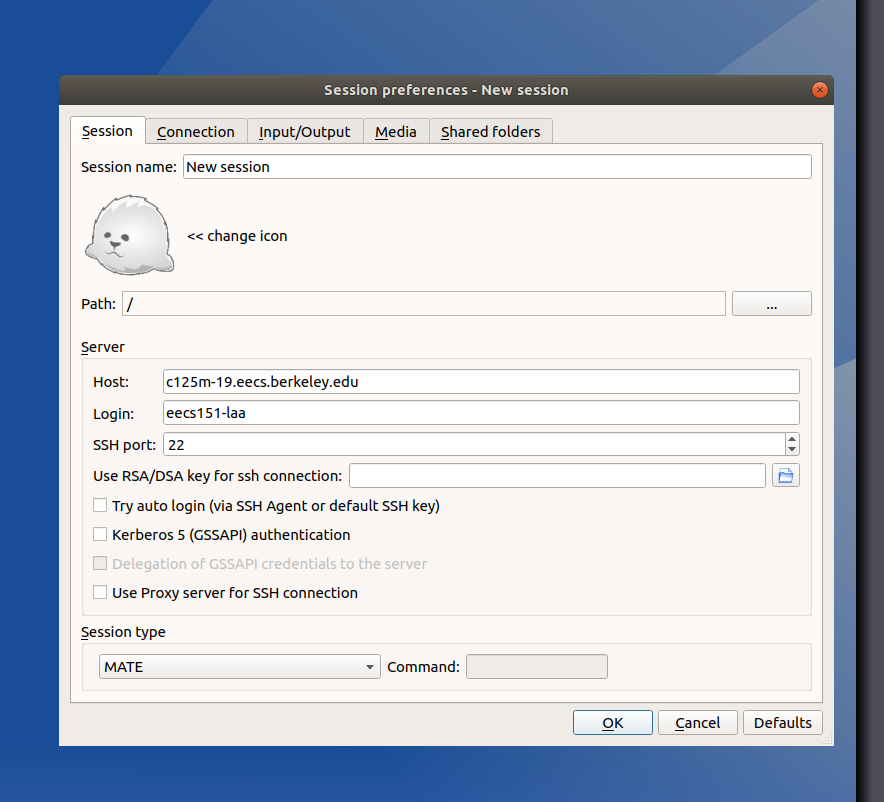
\includegraphics[width=0.55\textwidth]{figs/x2go_setup.png}
\end{center}

Once logged in using your class account and password, you should see a CentOS Linux desktop environment like the one below. This desktop is running on the lab machine of your choice and is being forwarded to you by x2go.

\begin{center}
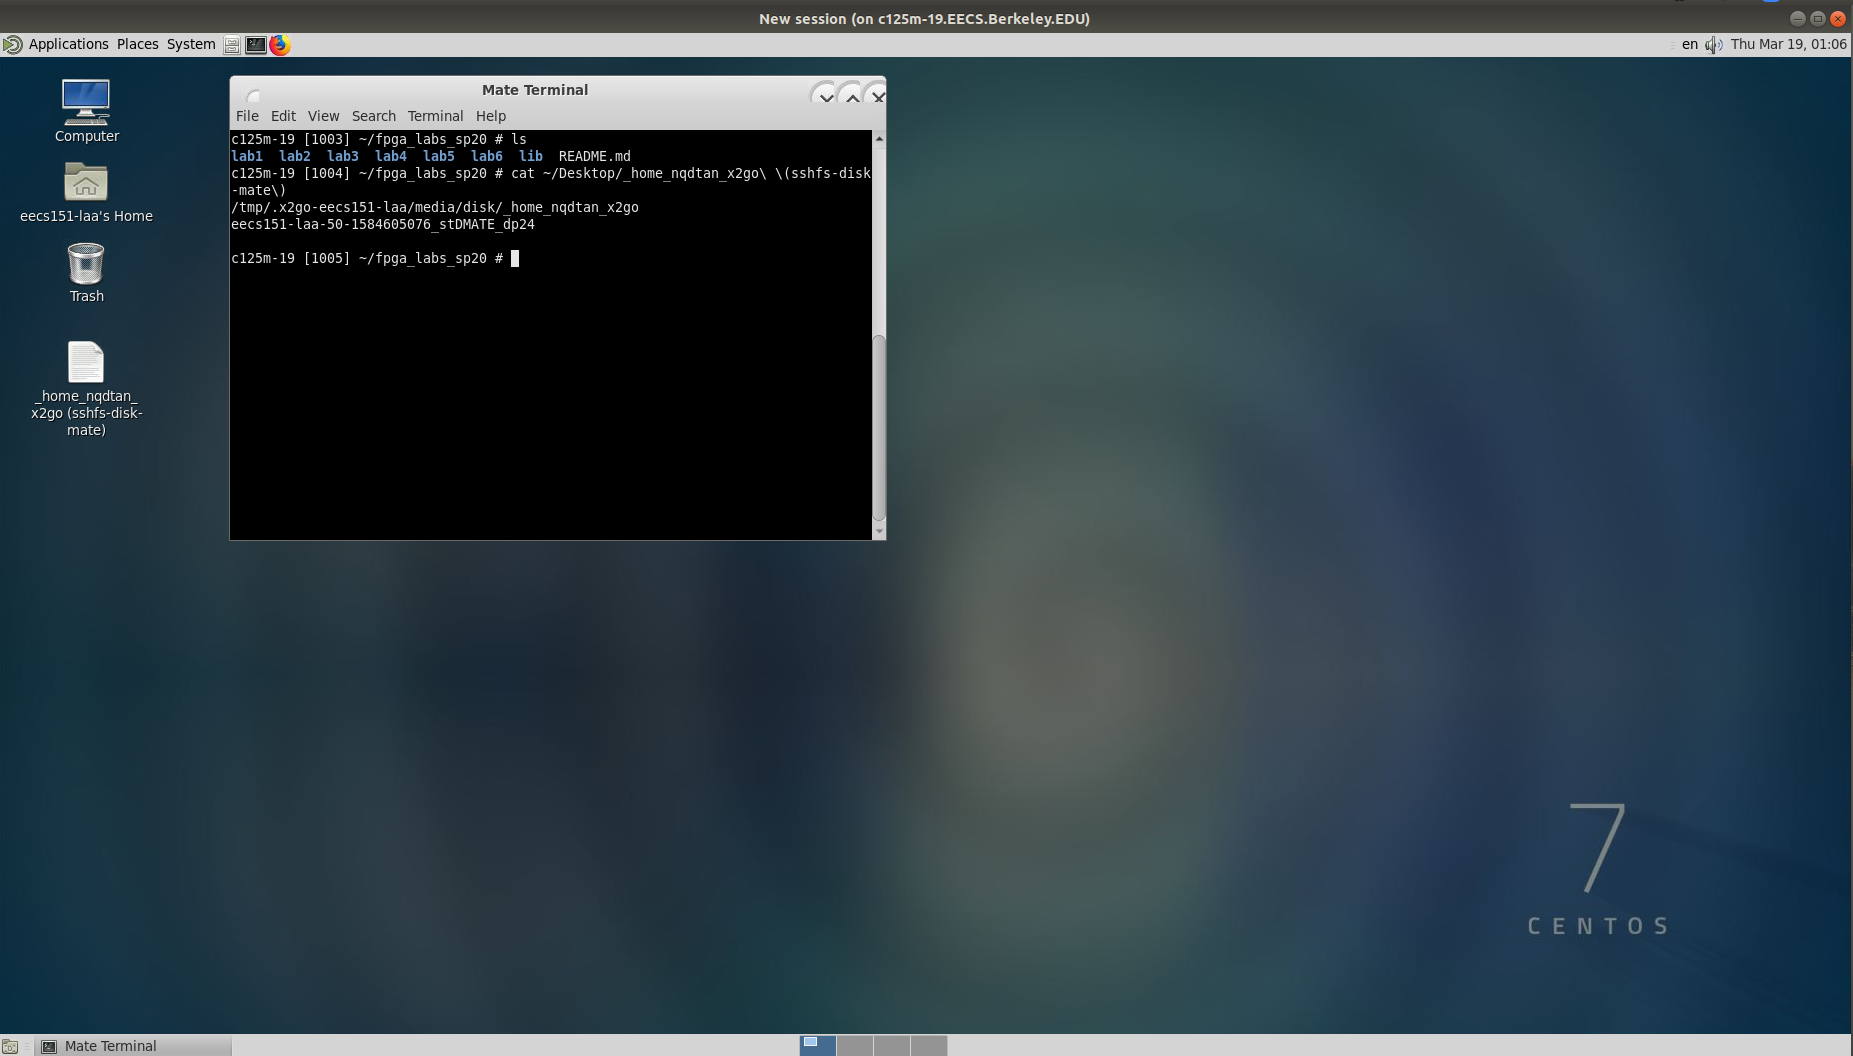
\includegraphics[width=0.55\textwidth]{figs/x2go_desktop.png}
\end{center}


\section{Getting Familiar with our Development Environment}
\subsection{Linux Basics}
In this class, we will be using a Linux development environment. We will be using CentOS as our Linux distro, which is a free version of Red Hat Linux. If you are unfamiliar or uncomfortable with Linux, and in particular, using the bash terminal, you should definitely check out this tutorial:

\url{https://www.digitalocean.com/community/tutorial_series/getting-started-with-linux}

It is highly recommended to go through all four parts of the tutorial above. To complete the labs and projects for this course, you will find it helpful to have good command line skills.

One of the best ways to expand your working knowledge of bash is to watch others who are more experienced. Pay attention when you are watching someone else's screen and ask questions when you see something you don't understand. You will quickly learn many new commands and shortcuts.

\subsection{Git Basics}
Please feel free to skip this section if you already have some prior experience with using git.

Version control systems help track how files change over time and make it easier for collaborators to work on the same files and share their changes. For projects of any reasonable complexity, some sort of version control is an absolute necessity. There are tons of version control systems out there, each with some pros and cons. In this class, we will be using Git, one of the most popular version control systems. It is highly recommended that you make the effort to really understand how Git works, as it will make understanding how to actually use it much easier. Please check out the following link, which provides a good high level overview:

\url{http://git-scm.com/book/en/Getting-Started-Git-Basics}

Once you think you understand the material above, please complete the following tutorial:

\url{http://try.github.com}

Git is a very powerful tool, but it can be a bit overwhelming at first. If you don't know what you are doing, you can really cause lots of headaches for yourself and those around you, so please be careful. If you are ever doubtful about how to do something with Git ask a TA or an experienced classmate.

For the purposes of this class you will probably only need to be proficient with the following commands:
\begin{itemize}
\item {\tt git status}
\item {\tt git add}
\item {\tt git commit}
\item {\tt git pull}
\item {\tt git push}
\item {\tt git clone}
\end{itemize}
However, if you put in the effort to learn how to use some of the more powerful features (diff, blame, branch, log, mergetool, rebase, and many others), they can really increase your productivity.

Git has a huge feature set which is well documented on the internet. If there is something you think Git should be able to do, chances are the command already exists. We highly encourage you to explore and discuss with fellow classmates and TA's.

\textit{Optional:} If you would like to explore further, check out the slightly more advanced tutorial written for CS250:

\url{http://inst.eecs.berkeley.edu/~cs250/fa13/handouts/tut1-git.pdf}

\section{Setting Up Github Access}
We will be using Github as our remote Git server for this class. Github is a popular Git hosting service which is home to many private and public (open-source) projects.

\subsection{SSH Keys}
Github authenticates you for access to your repository using ssh keys. Follow this tutorial to get SSH keys set up (this should be done on a lab workstation when you are logged in with your eecs151 class account).

First, create a new SSH key (do this on the lab computer):
\begin{verbatim}
ssh-keygen -t rsa -b 4096 -C "your_email@berkeley.edu"
\end{verbatim}
Keep hitting enter to use the default settings.

Then, from your terminal run:
\begin{verbatim}
cat ~/.ssh/id_rsa.pub
\end{verbatim}

Copy the public key that's printed out in its entirety. Go here: \url{https://github.com/settings/keys}, click on 'New SSH Key', paste your public key into the box, and click 'Add SSH key'.

Finally test your SSH connection: \url{https://help.github.com/articles/testing-your-ssh-connection/#platform-linux}.

If you have any issues, ask a TA for help.

\subsection{Acquiring Lab Files}
The lab files, and eventually the project files, will be made available through a git repository provided by the staff. The suggested way to obtain these files is as follows. First, set up your ssh keys as described above. Then run the command below in your home directory,

\begin{verbatim}
git clone git@github.com:EECS150/fpga_labs_sp21.git
\end{verbatim}

Whenever a new lab is released, you should only need to \verb|git pull| to retrieve the new files. Furthermore, if there are any updates, \verb|git pull| will fetch the changes and merge them in.

For now, you will only have pull access to this repository. If you create your own repository to store your code, make sure it's set to private to keep the code to yourself. Later on, each team will receive their own private repo for the final project, and you will be able to push and pull from that.

\section{Our Development Platform - Xilinx PYNQ-Z1}
\label{section:platform}

\subsection{Overview}

For the labs in this class, we will be using the Xilinx PYNQ-Z1 development board which is built on the Zynq development platform. Our development board is a printed circuit board that contains a Zynq-7000 System-on-Chip (SoC) along with a host of peripheral ICs and connections. The development board makes it easy to program the FPGA and allows us to experiment with different peripherals.

The best \href{https://reference.digilentinc.com/reference/programmable-logic/pynq-z1/reference-manual}{reference for this board} is provided by Digilent.
Browse the documentation there to get a feel for both what features the board has and, more importantly, what information the documentation has, should you need it later.

Being a development board, the silkscreen print clearly identifies connectors of interest. You should be able to recognize the most basic IO features on the board: GPIO LEDs, slide switches, and push-buttons. You should also be familiar with other basic elements of the board: input power socket, power switch, and the USB programming port. The following image identifies important parts of the board that may not have been obvious:

\begin{minipage}[h]{0.5\textwidth}
    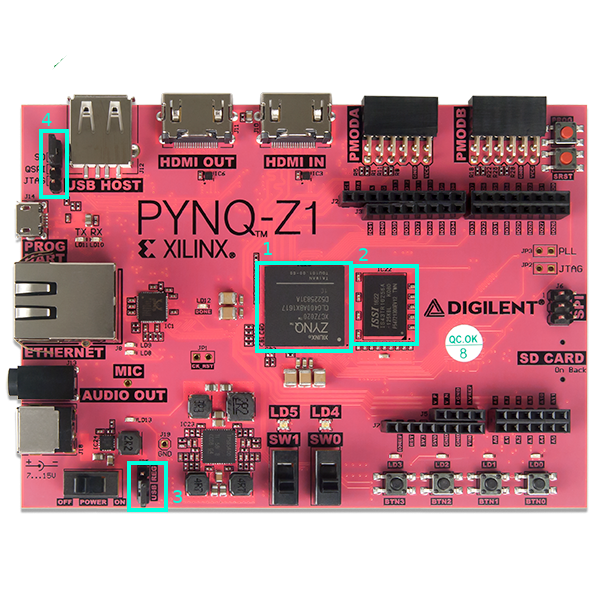
\includegraphics[width=\textwidth]{figs/z1_top_annotated.png}
\end{minipage}
\begin{minipage}[h]{0.5\textwidth}
    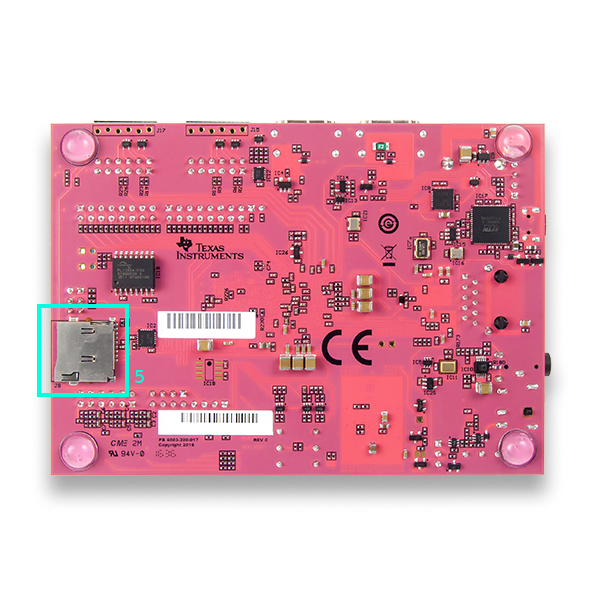
\includegraphics[width=\textwidth]{figs/z1_bottom_annotated.png}
\end{minipage}

\begin{enumerate}
  \item Z-7020 System-on-Chip (SoC) of the Zynq-7000 SoC family. It comprises a hardened dual-core ARM processor and the Xilinx FPGA xc7z020clg400-1. The SoC connects to the peripheral ICs and I/O connectors via PCB traces.
  \item ISSI 512MB off-chip DRAM.
  \item Power source jumper: shorting "REG" has the board use the external power adapter as a power source; shorting "USB" has it rely on the 5 V provided by USB. The latter will work unless your design needs to power a lot of external peripherals.
  \item Programming mode jumper to select how we want to use the ARM processor. There are two available modes: Operating-System mode (booting Linux from SD card) or Bare-metal mode. Since we are not using the ARM processor, we avoid this for now.
  \item SD card slot for inserting an SD card to boot Linux. Since we are not using the ARM processor, we avoid this for now.
\end{enumerate}

\subsection{The FPGA - xc7z020clg400-1}

xc7z020clg400-1 is the part ID of our FPGA. How should we interpret it? \texttt{xc7z020} is the part number which should help us to identify the specific device from a Xilinx FPGA family (in this case, it belongs to a Zynq family from the 7-series). \texttt{clg400} is the package number which defines how many package IO pins. \texttt{-1} is the speed grade.

Our FPGA is an Artix-7 Programmable Logic fabric which is a low-end 7-series Xilinx FPGA family (the mid-end and high-end of the 7-series are Kintex-7 and Virtex-7 families, respectively).
To help you become familiar with the FPGA that you will be working with through the semester, please skim Chapter 21: Programmable Logic Description of the \href{https://www.xilinx.com/support/documentation/user_guides/ug585-Zynq-7000-TRM.pdf}{Technical Reference Manual} and Chapter 2 of the \href{http://www.xilinx.com/support/documentation/user_guides/ug474_7Series_CLB.pdf}{Xilinx 7-series Configurable Logic Block User Guide}.
Pay particular attention to pages 15-25 on Slices and pages 40-42 on Multiplexers.
Please also read \href{https://www.xilinx.com/support/documentation/selection-guides/zynq-7000-product-selection-guide.pdf}{Zynq-7000 Product Selection guide}. Pay attention to slide 2. Can you identify our chip?

FPGA devices are usually attributed by their logic capacities. You should be aware of the device resource of your target FPGA when designing your digital circuit (it is unlike the software world where a CPU or GPU should be able to compile and run whatever code throwing at it regardless of the code size). Early FPGAs employ primitive blocks such as LUTs or FFs (Flip-flops) for logic implementation. Then the FPGA vendors started adding hardened blocks such as fast carry adders, block memories (BRAM) and Digital Signal Processing (DSP) slices onto FPGAs to augment their capability. The carry adder macros can implement fast arithmetic and comparison operations, the BRAMs provide fast on-chip storage, and the DSP slices are able to compute multipliers very efficiently, among many other operations. State-of-the-art FPGAs also incorporate floating-point calculation capability in those hardened blocks, thus greatly enhance the performance and expand their applicability. FPGA now has evolved to a competitive programmable platform, and there are many real-world applications that can be accelerated on the FPGAs, such as networking, wireless, biology, video/image processing, finance, or deep learning. The Zynq-7000 product line (which incorporates ARM processors next to a Programmable Logic -- as in the chip we are using right now) also provides a great platform for embedded applications.

You will need to answer the following questions in your lab report. Hint: read the documents mentioned above carefully.

\subsection{Your Task: Understanding your FPGA}\label{sec:fpgaQuestions}
\begin{enumerate}
  \item How many LUTs, FFs, Block RAMs (number of 36Kb blocks), and DSP slices are on the xc7z020 FPGA?
  \item How many SLICEs are in a single CLB? What does each SLICE contain?
  \item What is the difference between a SLICEL and a SLICEM?
  \item How many inputs do each of the LUTs have?
  \item How do you implement logic functions of 7 inputs in a single SLICEL? How about 8? Draw a high-level circuit diagram to show how the implementation would look. Be specific about the elements (LUTs, muxes) that are used.
\end{enumerate}

\section{Overview of the FPGA Build Toolchain}

Before we begin the lab, we should familiarize ourselves with the CAD (computer aided design) tools that translate a circuit implemented in a Hardware Description Language (such as Verilog) into a bitstream that configures the FPGA.
These tools will pass your design through several stages, starting with logic synthesis, followed by placement and routing. The final stage generates a bitstream ready to download to your FPGA.
In previous years, older evaluation platform (the ML505) used older FPGAs (a Xilinx Virtex-5 LX110T) and an older software suite (Xilinx ISE).

Our new boards use Xilinx's latest design software, the Vivado Design Suite which supports modern Xilinx FPGA devices, and features improved CAD algorithms to produce higher quality-of-result in shorter time.
Vivado also has integrated scripting capability (using the Tcl language -- pronounced "tickle") which allows users to write Tcl commands to interact with Vivado in a command-line fashion.
It is a great alternative to the GUI mode. A good way of learning the tool without relying on the GUI is to be aware of different Tcl commands, and how to use them. In the first few labs, we will learn how to use Vivado with the GUI mode. The subsequent labs will introduce necessary automated scripts and Makefile to improve our productivity.

Please ask a TA if you are unclear about any of the steps below.

\subsection{Set up your PYNQ-Z1}
\begin{enumerate}
  \item Plug in the power adaptor to power up the board.
  \item Connect the USB interface to a spare USB port on your workstation. Make sure you have installed Digilent cable driver if you use Vivado locally on your own machine.
  \item Turn the board on.
\end{enumerate}

Alternatively, you can also power up the board with the USB cable instead by switching the Power source jumper \texttt{JP5} position (see ~\ref{section:platform}). In this case, there is no need to use the power adaptor.

\subsection{Set up Vivado}

Before proceeding to the next section, you must make sure that you have access to the Vivado software (version \texttt{2019.1}) at this point.

If we were physically in the lab, this would have been no problem, since all the lab machines have Vivado installed. You can remotely access to any lab machine to run Vivado (via SSH, x2go, putty, etc.). To configure an FPGA board, we will send a bit file (a.k.a "bitstream") generated by Vivado through a USB cable to the board. There are several ways to accomplish this.

\begin{enumerate}
  \item Use the provided Virtual Box VM Image that has all the necessary toolchains installed for the labs (and the project). The VM offers similar development environment to the lab machines. This is the easiest option and it should work out-of-the-box regardless of which OS you are using on your home computer. The disadvantage is that it could consume a huge disk space (around 24 GB). Please check out Appendix~\ref{section:vm}.
  \item Install Vivado locally on your own machines. The Vivado WebPack version is free and it supports our FPGA device! This is also convenient if you have some disk space to spare (around 10 GB with the minimal installation option). Please check out Appendix~\ref{section:localvivado}.
  \item Use Vivado remotely, program the FPGA locally. This is the most adventurous road. Vivado Hardware Server is a minimal software program that can only be used to program an FPGA. Once you generate a bitstream file (e.g., remotely), you can either copy it to your own computer, and then use the Hardware Server to program your board. Alternatively, the Hardware Server also provides an option to download a bitstream to your board from a remote server. Please check out Appendix~\ref{section:localserver} for the installation steps and Section~\ref{section:hw_server} for how to program the FPGA from remote server.
\end{enumerate}

If you follow either option (2) or (3), you will need to install the required drivers so that your machine can recognize the board (unless you use the VM with Hardware Server intalled). Please read Appendix~\ref{section:localvivado} for the instruction of how to do so.

The third option is recommended if your network connection to the lab machines is stable most of the time. If you have time, you may want to explore the options to see which one works best for your case.

Again, please make sure you have Vivado ready before moving on.

\subsection{Verilog source file}
Throughout the semester, you will build increasingly complex designs using Verilog, a widely used hardware description language (HDL).

Open up the \verb|lab1/src/z1top.v| source file.
This file contains a Verilog module description which specifies input and output signals. It also describes the logic gate connecting the signals (just a single AND-gate!).

Next, open up the constraint file in \verb|lab1/constr/z1top.xdc|.
This file, which contains several Tcl commands, specifies some IO pin mappings. Note how the signals in the Verilog code correlate with the pin-mapping commands in this file.

Let's see one example:

\begin{minted}{tcl}
set_property -dict { PACKAGE_PIN M20 IOSTANDARD LVCMOS33 } [get_ports a];
\end{minted}

This syntax assigns the properties \verb|PACKAGE_PIN| and \verb|IOSTANDARD| with the values \verb|M20| and \verb|LVCMOS33| (respectively) to the port \verb|a|, a signal we defined in our Verilog source. Each of these properties has a separate consequence in the synthesis process:

\begin{itemize}
  \item The pin to which the \verb|a| signal should be connected to the physical pin M20 on the FPGA package.
  \item The logic convention (maximum voltage, what ranges constitute low and high, etc) for that port will be LVCMOS33.
\end{itemize}

To understand the peripheral to which pin M20 connects on the PYNQ-Z1 board, you should inspect page 9 of the \href{https://reference.digilentinc.com/_media/reference/programmable-logic/pynq-z1/pynq-z1\_sch.pdf}{PYNQ-Z1 schematic}. Based on the pin assignments described in the constraint file, our logic circuit performs an AND function of the two Switches (SW0 and SW1) on the board, and the result is shown on the LED 0 (LD0).

Setting constraints is one of the most important steps in the FPGA development flow, especially if your circuit interfaces with the external world (receiving signals or sending signals via IO circuitry of the board). Please do not forget this step. You will not be able to generate a bitstream if you do not set the pin mapping to all the input/output signals of your top-level Verilog module; Vivado will complain and abort. More importantly, your FPGA design will not work properly if your pin assignment is wrong. A good practice is to check the documentation/schematic of your target FPGA device carefully of which IO peripheral maps to which pin, and the appropriate logic standard unless you can get the sample board constraint file from the vendor.

Let's put this digital circuit on the FPGA! In the next section, we will learn how to create a basic Vivado project, add our Verilog and constraint files, and generate a bitstream file to program our FPGA.

\subsection{Creating Vivado Project}

This section describes how to create a Vivado project using GUI mode. Project is a neat and organized way of managing your RTL design and constraint files, exercise different design steps, generate a bitstream to configure an FPGA, or review the design reports.

In our CentOS environment, press \texttt{Alt + F2} to bring up a command dialog. Type the full path to the \texttt{vivado} binary to open Vivado GUI locally in your machine:

\begin{verbatim}
/opt/Xilinx/Vivado/2019.1/bin/vivado
\end{verbatim}

(You can also run this from a terminal or create a Desktop shortcut.)

We suggest that you add the following command to your \texttt{.bashrc} file, so that you only need to type \texttt{vivado} instead of the full path to launch Vivado.

\begin{minted}{bash}
source /opt/Xilinx/Vivado/2019.1/settings64.sh
\end{minted}

Create new project by select \emph{File} $\rightarrow$ \emph{New} $\rightarrow$ \emph{Project} to launch the following wizard.

\begin{center}
\fbox{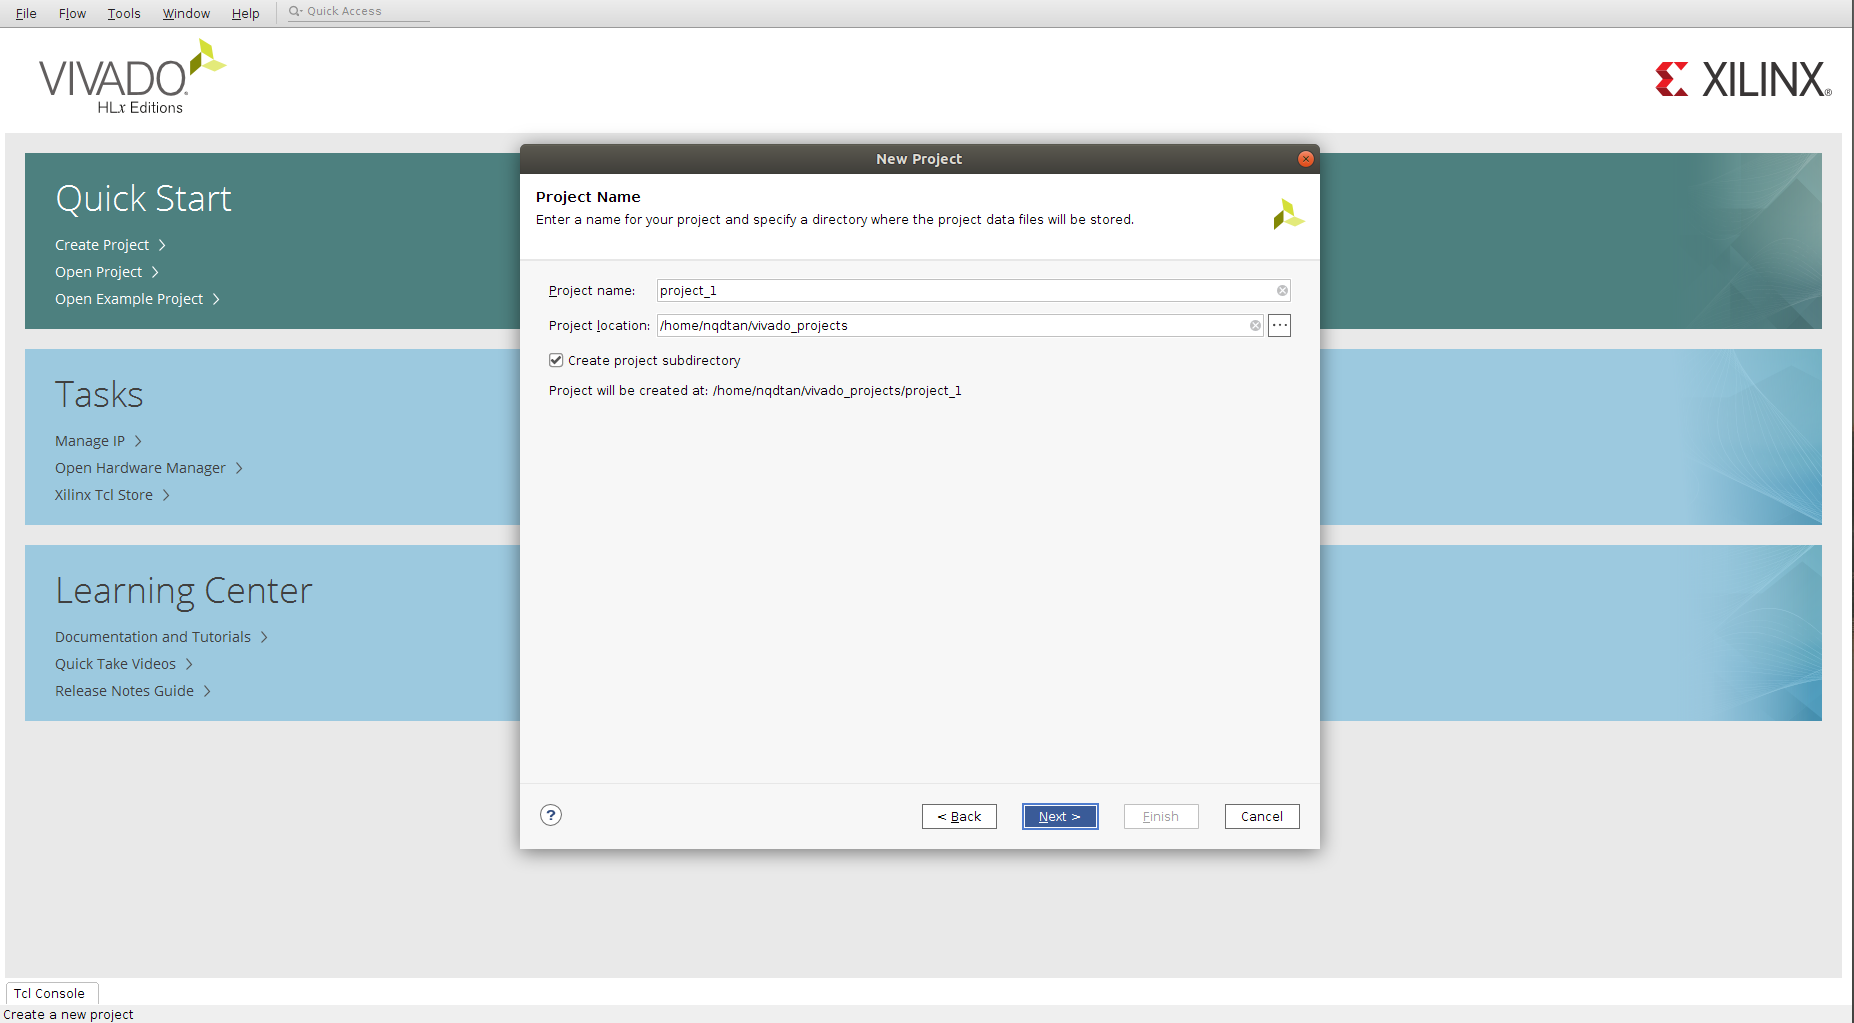
\includegraphics[width=0.7\textwidth]{figs/vivado0.png}}
\end{center}

Type the project name and location. You can leave them as default. Click \emph{Next}. In the next window, make sure to select \emph{RTL project}, and \emph{Do not specify sources at this time}.

\begin{center}
\fbox{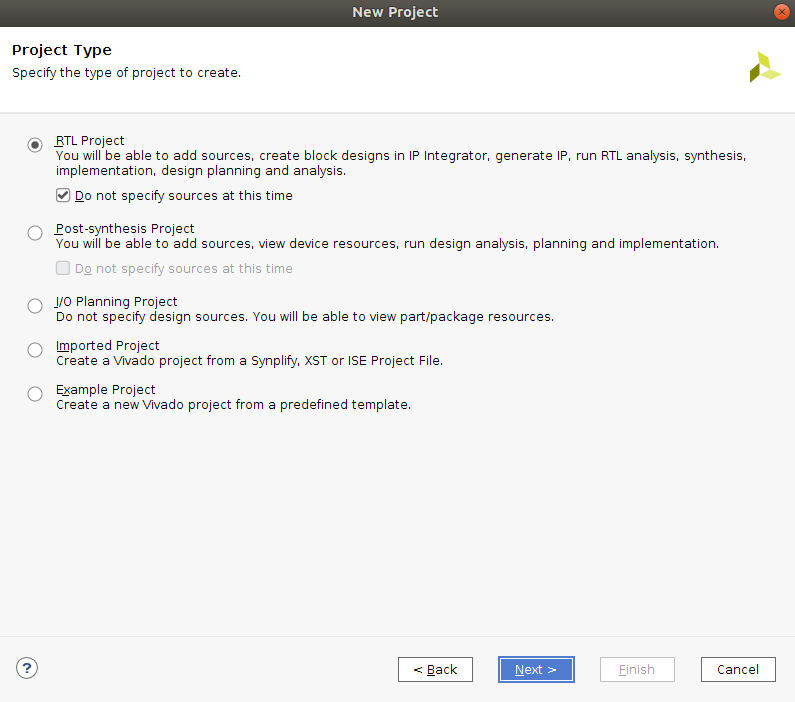
\includegraphics[width=0.4\textwidth]{figs/vivado1.png}}
\end{center}

Next, we select the target FPGA device for the project. Click the \emph{Boards} tab, find the PYNQ-Z1 entry and select it.

\begin{center}
\fbox{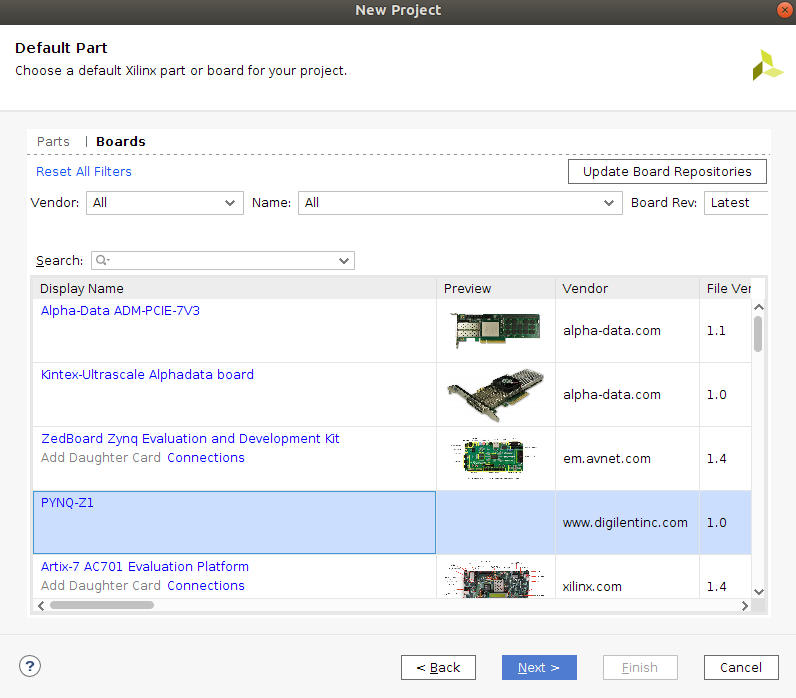
\includegraphics[width=0.4\textwidth]{figs/vivado2.png}}
\end{center}

If you cannot find the PYNQ-Z1 entry, chance is your Vivado installation does not include the PYNQ-Z1 board files. Follow the instructions from \href{https://pynq.readthedocs.io/en/v2.3/overlay_design_methodology/board_settings.html#vivado-board-files}{Vivado board files} to add the PYNQ-Z1 files to your Vivado installation (or read Appendix~\ref{section:localvivado}).
Alternatively, you can select the part ID xc7z020clg400-1 from the \emph{Parts} tab as follows.

\begin{center}
\fbox{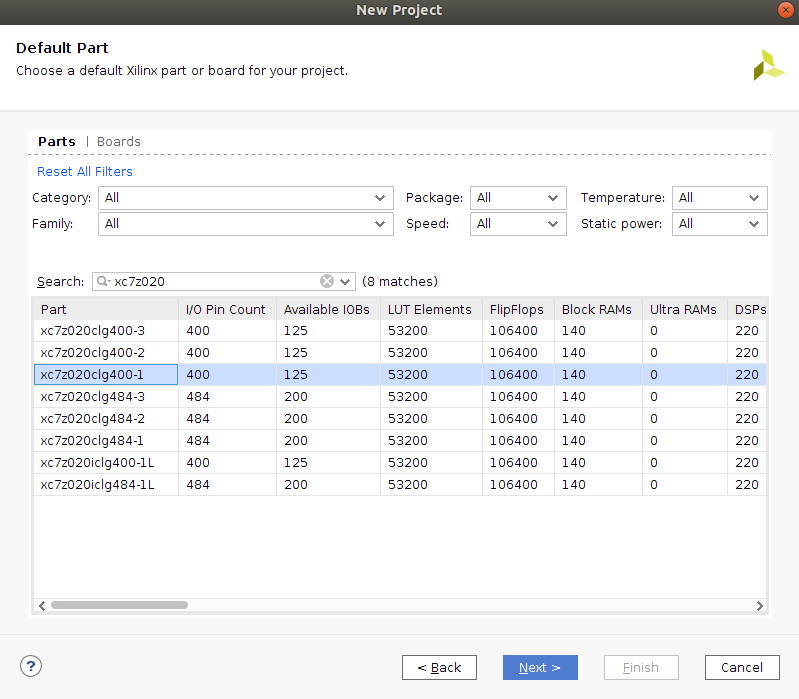
\includegraphics[width=0.4\textwidth]{figs/vivado2_1.png}}
\end{center}

Once you are done, you should be able to see a window as follows.

\begin{center}
\fbox{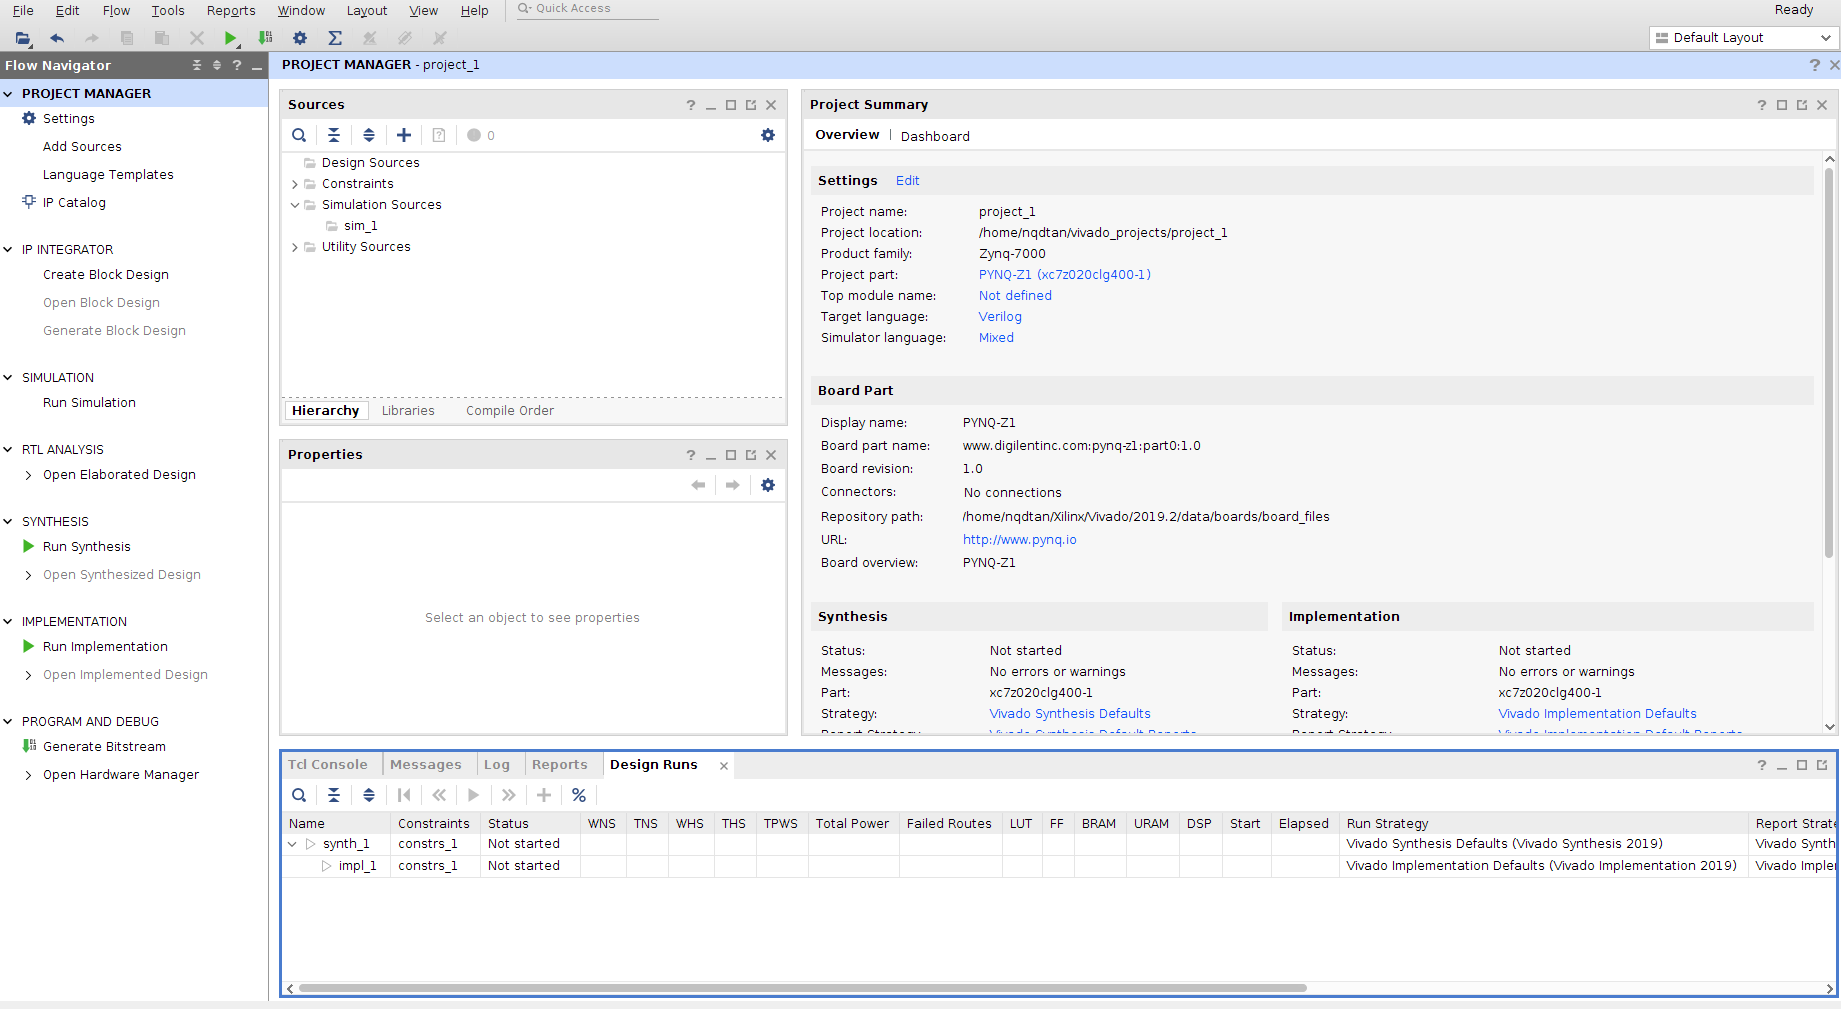
\includegraphics[width=0.7\textwidth]{figs/vivado3.png}}
\end{center}

Now we start adding our design and constraint files to the project. Press \texttt{Alt + A} to add files as follows (or right click on the Sources pane and select \emph{Add Sources}).

\begin{center}
\fbox{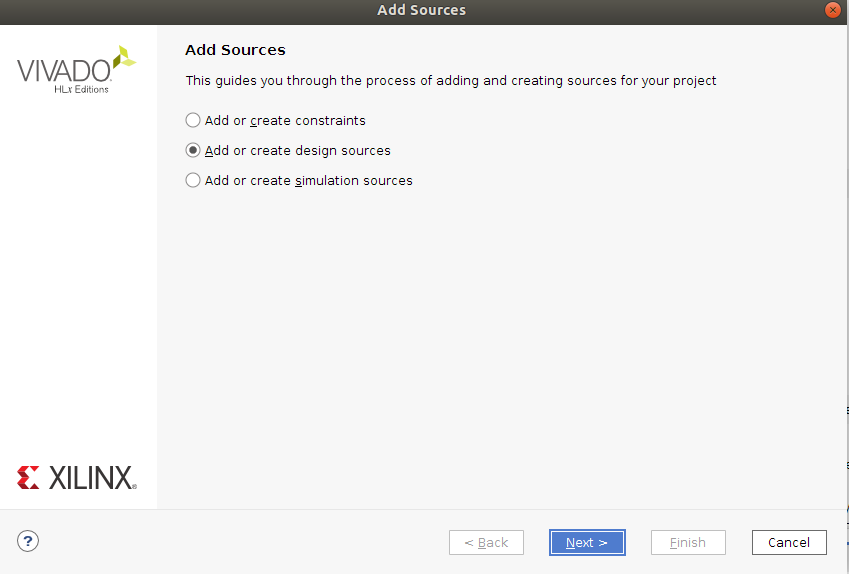
\includegraphics[width=0.4\textwidth]{figs/vivado4.png}}
\end{center}

Add your Verilog source file(s).

\begin{center}
\fbox{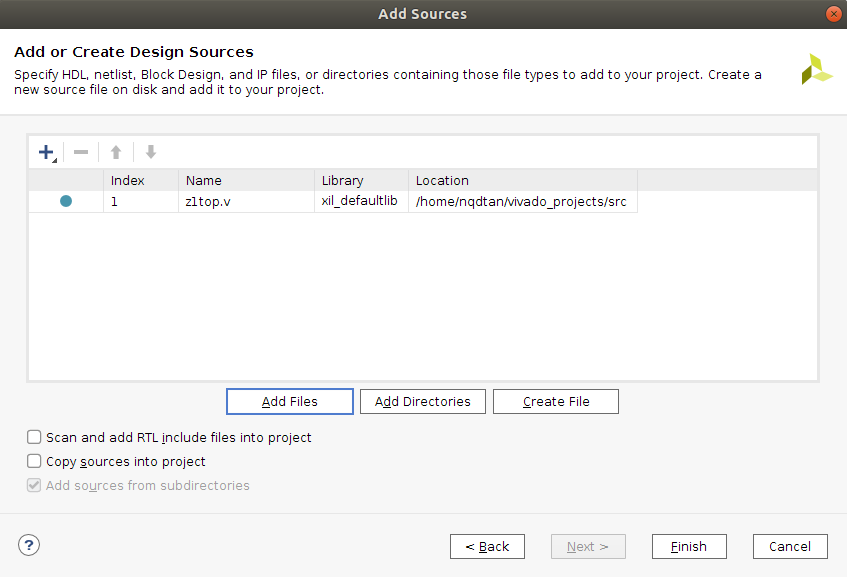
\includegraphics[width=0.4\textwidth]{figs/vivado5.png}}
\end{center}

And repeat the step to add your constraint file.

\begin{center}
\fbox{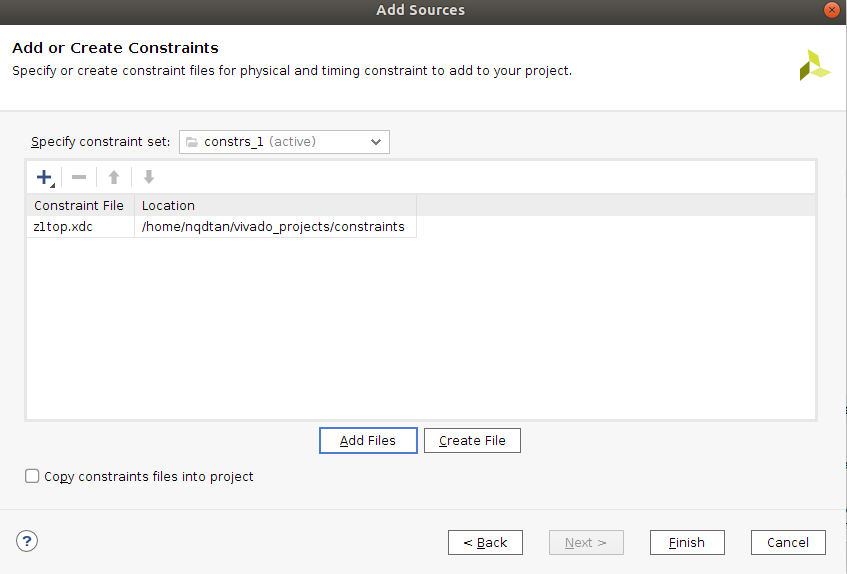
\includegraphics[width=0.4\textwidth]{figs/vivado6.png}}
\end{center}

Our first Vivado project is good to go now! Note that you can also use Vivado code editor to write Verilog code. This might be a good starting point if you first learn the language since the tool is able to capture syntax errors or obvious bugs quickly which could save you from a lot of potential miseries down the road.

\begin{center}
\fbox{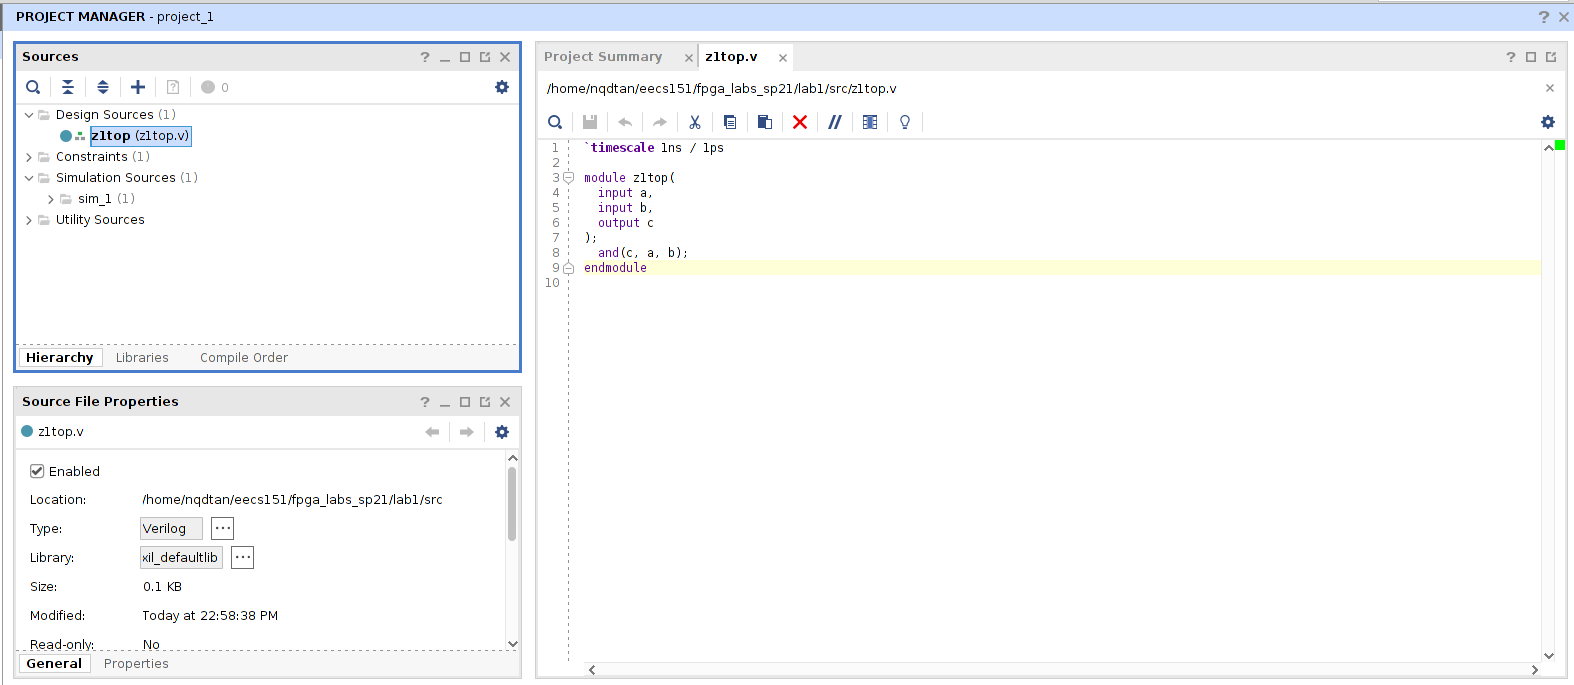
\includegraphics[width=0.7\textwidth]{figs/vivado_code.png}}
\end{center}

Note where Vivado creates a project directory in your system. If you close your Vivado project and want to reopen it, type

\begin{minted}{bash}
vivado /path/to/{vivado_project_dir}/{project_name}.xpr
\end{minted}

The default project name is \texttt{project\_1}.

\subsection{Synthesis}
The Synthesis step performs logic synthesis which translates the input HDL code into a netlist of FPGA primitives such as LUTs, FFs, BRAMs, or DSPs. Remember that there is no logic gate at all in an FPGA! To run the synthesis step in the Vivado Design Suite, select \emph{Run Synthesis} in the \emph{Flow Navigator} pane on the left-hand side of the window. If this had been run before, the synthesized design can be inspected by selecting \emph{Open Synthesized Design}. Select \emph{Schematic} under ``Open Synthesized Design" on the left toolbar to see a circuit schematic.

If you wish to see the circuit netlist in the form of Verilog, type the following Tcl command

\begin{minted}{tcl}
write_verilog my_netlist.v
\end{minted}

in the \emph{Tcl Console} at the bottom pane. Check that the AND gate has now mapped to a 2-input LUT.

\subsection{Implementation}
The Implementation step performs placement and routing of the design. Placement places the primitives in the netlist to the physical locations on the FPGA. Routing connects the placed blocks together using switch blocks and wires on the FPGA. The next step is timing analysis which evaluates if your design meets the target clock constraint (this only applies if your design has sequential elements, such as Flip-flops or Block RAMs). Implementation is the most time-consuming task of a hardware design flow, especially if you have a complex design. Select \emph{Run Implementation} in the \emph{Flow Navigator} to run it, then select \emph{Open Implementation}. You should be able to see the device floorplan of the FPGA chip now. Can you locate the LUT cell that implements our original 2-input AND gate? You might need to zoom in the floorplan view to find it. Click \emph{Routing Resources} button on the menu bar to toggle the display of the routing wires that connect the IO pins and the LUT.

\subsection{Generate Bitstream and Program FPGA}
To generate the bitstream for our target FPGA, we invoke \emph{Generate Bitstream} in the \emph{Flow Navigator}. This step will generate a *.bit file that programs the FPGA. Different FPGA chips will requires different bitstream formats. Therefore, make sure that you always set the correct target device/board (to PYNQ-Z1 -- as always for our labs) when creating a Vivado project.

\textbf{Please note: this step assumes that you can generate a bitstream from Vivado locally (either by using the VM with full Vivado software or installing Vivado locally on your own machine).}

When the bitstream generation is done, select \emph{Open Hardware Manager} and connect to your FPGA. If you haven't before, or the hardware manager says no devices are connected, select \emph{Menu} $\rightarrow$ \emph{Open New Target}. In the Hardware Server Setting, make sure you pick \emph{Local server} (if you are using Vivado locally). You should see \verb|xilinx_tcf| listed under Harware Targets in the top pane. In the bottom pane, two entries: \verb|arm_dap_0| and \verb|xc7z020_1|. That's good. \emph{Next} $\rightarrow$ \emph{Finish}.

\begin{center}
\fbox{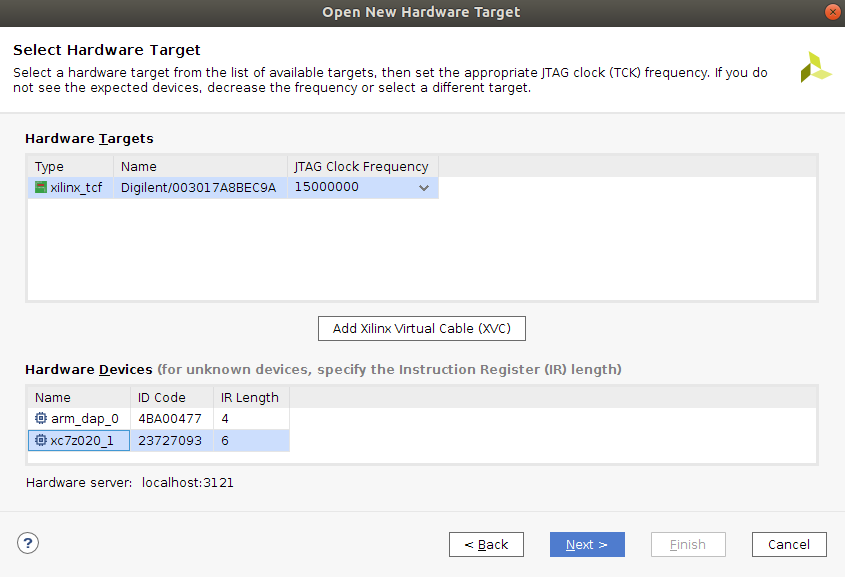
\includegraphics[width=0.7\textwidth]{figs/vivado10.png}}
\end{center}

If you don't see any hardware targets, it might be due to missing drivers. Please check out the Appendix~\ref{section:localvivado} for how to install the drivers so that your system can recognize the board.

Next, click \emph{Program device} to load the bitstream to your connected FPGA. The "Done" LED (near the Zynq chip) should be on if you successfully configure the FPGA.

\begin{center}
\fbox{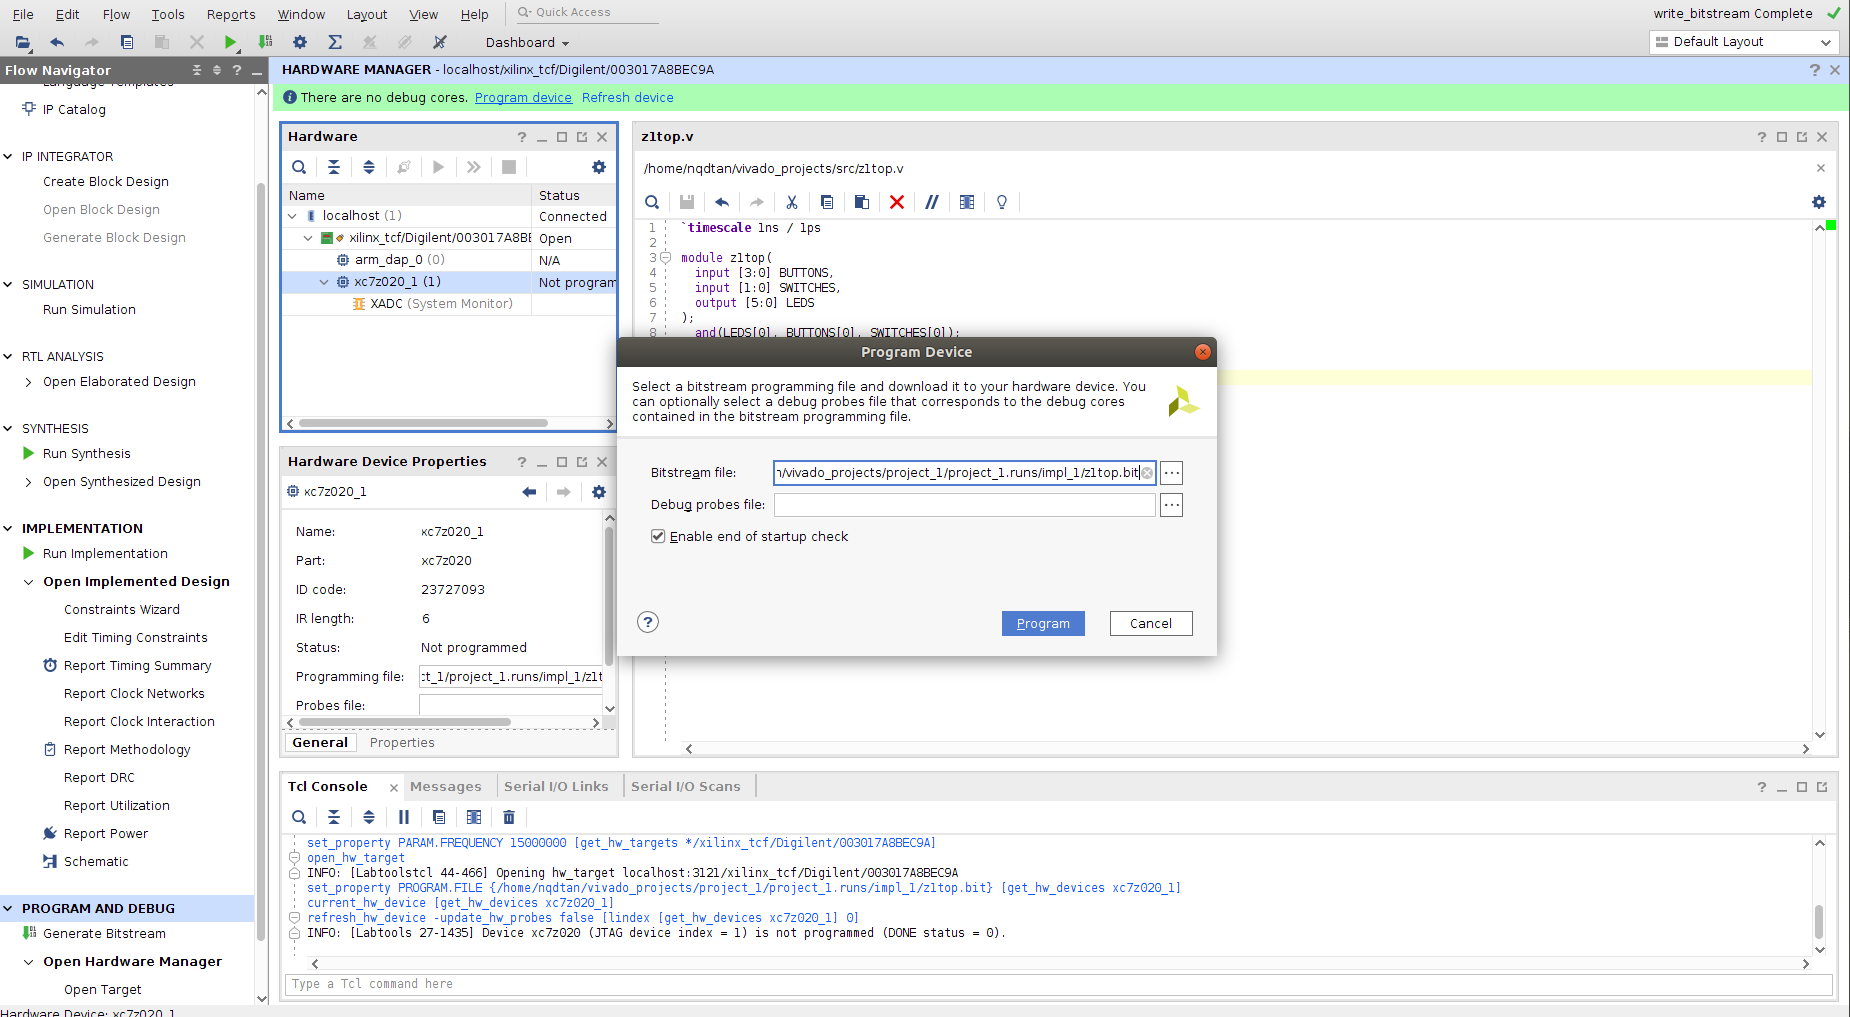
\includegraphics[width=0.7\textwidth]{figs/vivado11.png}}
\end{center}

See if it worked! What happens when you change the switches (SW0, SW1)?

Please don't be hesitate to ask a TA for help if you get stuck in any technical issues!

\section{Program FPGA with the Vivado Hardware Server}
\label{section:hw_server}

You can skip this section if you have Vivado locally on your computer (either by using the VM or installing Vivado yourself).

If we were physically using the lab machines, we'd now be able to program the bitstream onto our FPGA with a couple clicks. However, since we're using the lab machines remotely, we'll set up our computers as a relay so that the lab machines can program our locally connected FPGAs through the Internet. We do this by running Vivado Hardware Server, a subcomponent of the Vivado software, locally, and setting up an SSH reverse tunnel. We recommend using the VM that we have set up for you, but if you have any difficulties it is also possible to install the Vivado Hardware Server directly onto your computer if you're using Linux or Windows (see Appendix~\ref{section:localserver}).

\subsection{Installing the VM (with Hardware Server only)}
\label{section:vm}
For convenience, we've prepared a virtual machine image with Vivado Hardware Server already installed. There are two versions.

\begin{itemize}
\item GUI: \url{https://drive.google.com/file/d/1S0duf_oHfXs9fImsqNypIvR-nmrZuDca/view?usp=sharing}
\item Command line-only: \url{https://drive.google.com/file/d/133YZzW4nnEgabDuhmfxPH3ncQPwQPaVP/view?usp=sharing}
\end{itemize}

The command line-only version requires less computational resources, but is slightly less convenient. We'll be using the VM in a limited capacity (i.e. not for coding), so choose this version if performance is important for you.

To use the VM, install \href{https://www.virtualbox.org/}{VirtualBox}. Import the downloaded VM image and start it. The VM runs CentOS 7, like the lab computers. The username is \texttt{eecs151} and the password is \texttt{eecs151}.

The VM sets up USB filtering to recognize the devices we use for this class. For VirtualBox on Linux, if the USB devices (FPGA and UART) don't map into the VM, then be sure your account is in the "vboxusers" group (and log-off and back-on). For example, Ubuntu users can use the following command:

\begin{verbatim}
  sudo usermod -a -G vboxusers $USER
\end{verbatim}

\subsection{Running the Hardware Server}

In the VM, run the executable at \verb|/opt/Xilinx/HWSRVR/2019.1/bin/hw_server|.

\subsection{Setting Up an SSH Reverse Tunnel}
We now have to set up a connection through the Internet from our lab workstation to the machine running the hardware server.

In order to prevent collisions between multiple students using the same lab server, each student has been assigned a unique port number to use. Check the following sheet for your port number:

\href{https://docs.google.com/spreadsheets/d/1BeXS-TKXfxFqZ8cCp3gJYv2zRsh1nRchLU5TO5UcIkc/edit?usp=sharing}{FPGA Lab SP21 Server Port Assignments}

If you're not on this list, ask a TA.

In a new terminal (also in the VM), run the following, where \texttt{<your port>} is your port number from the sheet, \texttt{eecs151-xxx} is your class account and \texttt{c125m-x} is the lab machine you're using:

\begin{verbatim}
  ssh -R <your port>:localhost:3121 eecs151-xxx@c125m-x.eecs.berkeley.edu
\end{verbatim}

The \texttt{-R} flag indicates that this is a reverse tunnel connecting port \texttt{<your port>} of the lab machine to port \texttt{3121} of our local machine. 
If you only have a command line interface, \texttt{tmux} is a useful linux tool that can help you open multiple terminal sessions at once. 
The following tutorial explains how to use \texttt{tmux} to open two different terminals, in which you can run the above two commands:
\url{https://www.hamvocke.com/blog/a-quick-and-easy-guide-to-tmux/}

Here's an example of running the two commands side by side in \texttt{tmux}.

\begin{center}
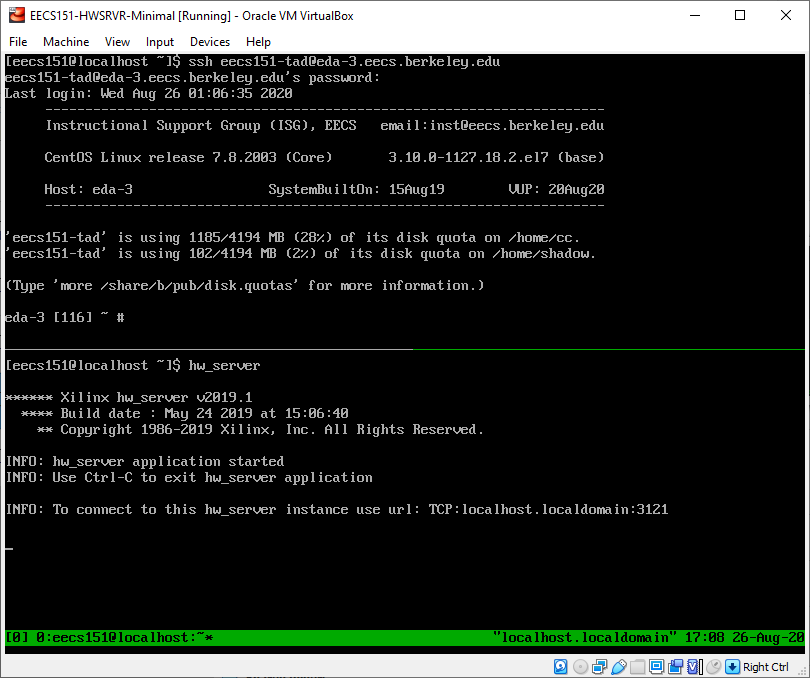
\includegraphics[width=0.8\textwidth]{figs/hwsrvr_vm.png}
\end{center}

Make sure you have connected and turned on the board at this point.

\subsection{Programming the FPGA}
Now, in Vivado on the \textbf{lab machine}, \emph{Open Hardware Manager} and connect to your FPGA. 
To do this, select \emph{Open Target} $\rightarrow$ \emph{Open New Target}. 
In the \emph{Open New Hardware Target} dialog, choose to connect to a \emph{Remote server} at Host name \texttt{127.0.0.1} and your assigned port number from before.

You should see \verb|xilinx_tcf| listed under Hardware Targets in the top pane. In the bottom pane, two entries: \verb|arm_dap_0| and \verb|xc7z020_1|. You're connected! \emph{Next} $\rightarrow$ \emph{Finish}, then \emph{Program Device}.

If you don't see any Hardware Targets, go back to your VM window, on the bottom-right corner, locate the \emph{USB Settings} icon, try turning off and on the `Digilent Adept USB Device'. Then try \emph{Open Target} again on the lab machine.

\section{Design Reports and Logs}

Reports are automatically generated at each step in the Vivado build flow. You should be able to discover them under each of the expanded stages in the \emph{Flow Navigator}. The \emph{Project Summary} window (under the \emph{Window} menu) presents a nice summary of the reports generated through each step. The reports tell you the Quality of Result (QoR) of your design, such as how many LUTs, FFs, BRAMs, DSPs are used, and whether your circuit meets the target clock constraint. 
You can open the reports from your terminal using your favorite text editor. The following reports are particularly important and you should pay attention to when evaluating, debugging, or optimizing your design.

\verb|project_1/project_1.runs/synth_1/z1top_utilization_synth.rpt|: Resource utilization report after synthesis.

\verb|project_1/project_1.runs/impl_1/z1top_utilization_placed.rpt|: Resource utilization report after placement.

\verb|project_1/project_1.runs/impl_1/z1top_utilization_routed.rpt|: Timing summary report after routing.

You will often find the log files helpful when you want to look for more information of how your Verilog code is compiled to a bitstream. Make sure you get what you want (if not, why) by putting effort in understanding the messages as well as warnings or errors if any from the log files.

\verb|project_1/project_1.runs/synth_1/runme.log|: Execution log of the synthesis step.

\verb|project_1/project_1.runs/impl_1/runme.log|:  Execution log of the implementation step.

\section{Lab Deliverables}
\subsection{Lab Checkoff (due: 11AM, Wednesday Feb 3rd, 2021)}
To checkoff for this lab, have these things ready to show the TA:
\begin{enumerate}
  \item Demonstrate that you can generate a bitstream from the given sample code using Vivado. In addition, please show that you can program your FPGA board correctly.
  \item Modify the sample code to implement a 4-input logic function of your choice. The inputs are the four buttons (BTN 0-3), and the output is LED 1 (LD1). Demonstrate that your logic circuit works correctly on the FPGA board. Make sure to inspect the PYNQ schematic (or \href{https://reference.digilentinc.com/_media/reference/programmable-logic/pynq-z1/pynq-z1_c.zip}{sample board constraint file}) to know the correct pin mappings for the Buttons and the LEDs, and then update the design and constraint files properly.
\end{enumerate}

\subsection{Lab Report (due: 11.59PM, Wednesday Feb 3rd, 2021)}\label{sec:labreport}
Also please submit a short lab report to Gradescope in which you answer/show the following things:
\begin{enumerate}
  \item Answers for the questions in section \ref{sec:fpgaQuestions}
\end{enumerate}


\newpage
\appendix
\appendixpage
\section{Installing the VM (with full Vivado Installation)}
\label{section:vm}
We provide a VirtualBox VM with CentOS 7 and Vivado 2019.1 WebPACK, which provides the full Vivado toolchain, installed. The download is about 10 GB and the VM expands to about 24 GB when imported into VirtualBox.

\url{https://berkeley.box.com/s/s4z0ykpf0tudrm9hce8fsmitpgb2khhe}

To use the VM, install \href{https://www.virtualbox.org/}{VirtualBox}. Import the downloaded VM image and start it. The VM runs CentOS 7, like the lab computers. The username is \texttt{eecs151} and the password is \texttt{eecs151}.

The VM sets up USB filtering to recognize the devices we use for this class. For VirtualBox on Linux, if the USB devices (FPGA and UART) don't map into the VM, then be sure your account is in the "vboxusers" group (and log-off and back-on). For example, Ubuntu users can use the following command:

\begin{verbatim}
  sudo usermod -a -G vboxusers $USER
\end{verbatim}

If you are a Mac user and have issue with the Hardware Manager (keep getting disconnected after some time), try enabling USB3.0 setting in your VM setting to see if it helps. To do so, first, please download the \href{https://www.oracle.com/virtualization/technologies/vm/downloads/virtualbox-downloads.html#extpack}{VirtualBox Extension Pack}. Next, please follow this \href{https://techspite.com/how-to-install-virtualbox-extension-pack-and-enable-usb-3-0-2/}{guide} to enable USB3.0 in VirtualBox.

\section{Installing Vivado Locally}
\label{section:localvivado}

Vivado can take up up to around 60 GB of disk space during the installation process, so make sure you have enough disk space available before installing locally.

Before doing this, you will need to register a (free) Xilinx account.

\subsection{Linux}
Create an install area for Vivado:
\begin{minted}{bash}
  sudo mkdir /opt/Xilinx
  sudo chmod 775 /opt/Xilinx
  sudo chown `whoami`:`whoami` /opt/Xilinx
\end{minted}

Download the `Vivado HLx 2019.1: WebPACK and Editions - Linux Self Extracting Web Installer' from the `Vivado Design Suite - HLx Editions - 2019.1  Full Product Installation' Linux bin from \href{https://www.xilinx.com/support/download/index.html/content/xilinx/en/downloadNav/vivado-design-tools/archive.html}{Xilinx}.

Execute the downloaded script.

\begin{minted}{bash}
  chmod +x Xilinx_Vivado_SDK_Web_2019.1_0524_1430_Lin64.bin
  ./Xilinx_Vivado_SDK_Web_2019.1_0524_1430_Lin64.bin
\end{minted}

During the install process, specify \texttt{/opt/Xilinx} as the install directory.
Also, you should only select the install options we're going to use in this class to save disk space:

\begin{center}
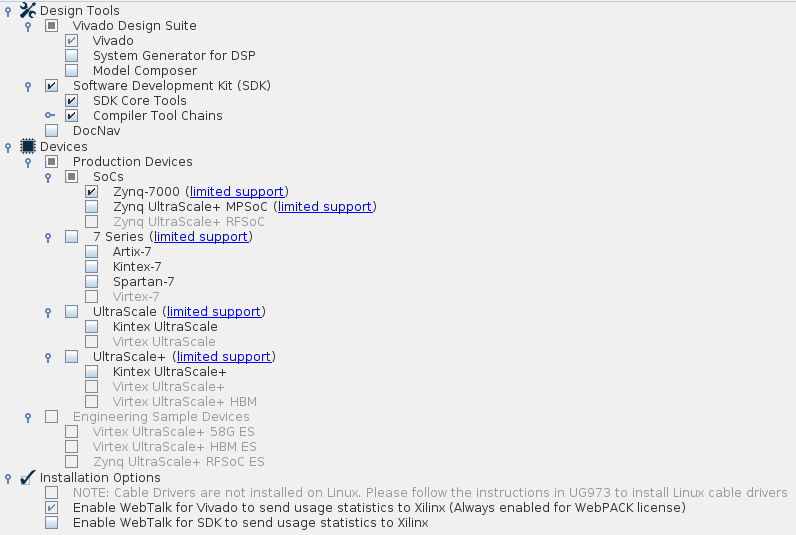
\includegraphics[width=0.7\textwidth]{figs/vivado_install_options.png}
\end{center}

During the install process, specify \texttt{/opt/Xilinx} as the install directory (or wherever works in your system)

After it's done, install the Digilent drivers to program the Pynq over USB-JTAG.
\begin{minted}{bash}
  cd /opt/Xilinx/Vivado/2019.1/data/xicom/cable_drivers/lin64/install_script/install_drivers
  sudo ./install_drivers
\end{minted}

You also need to add PYNQ-Z1 board files to Vivado since it does not have PYNQ support initially.
This allows you to set PYNQ-Z1 as the target platform when you create a Vivado project.

Download the following file \url{https://github.com/cathalmccabe/pynq-z1_board_files/raw/master/pynq-z1.zip}.

Extract and copy the \verb|pynq-z1| folder to

\texttt{<your Vivado installation directory>/Vivado/<version>/data/boards/board\_files}

\subsection{Windows}
Download the `Vivado HLx 2019.1: WebPACK and Editions - Windows Self Extracting Web Installer' from the `Vivado Design Suite - HLx Editions - 2019.1  Full Product Installation' Linux bin from \href{https://www.xilinx.com/support/download/index.html/content/xilinx/en/downloadNav/vivado-design-tools/archive.html}{Xilinx}.
Execute the downloaded exe.
Also, you should only select the install options we're going to use in this class to save disk space, as described in the Linux section.

If you have a driver issue when connecting the board to your computer, please follow this guide to see if it helps: \href{https://forums.xilinx.com/t5/Design-and-Debug-Techniques-Blog/Manually-installing-Cable-Drivers-for-Xilinx-Platform-Cable-USB/ba-p/992593}{Installing Cable Drivers}

\section{Installing Vivado Hardware Server Locally}
\label{section:localserver}

We recommend that you use the provided VM, but it is also possible for Linux and Windows users to install Vivado Hardware Server natively to their computer.

\subsection{Linux}
First, create an install area:
\begin{minted}{bash}
  sudo mkdir /opt/Xilinx
  sudo chmod 775 /opt/Xilinx
  sudo chown `whoami`:`whoami` /opt/Xilinx
\end{minted}

Download the `Vivado 2019.1 64-bit Hardware Server for Linux' (or 32-bit, if necessary) TAR file from \href{https://www.xilinx.com/support/download/index.html/content/xilinx/en/downloadNav/vivado-design-tools/archive.html}{Xilinx}.
You will need to create a Xilinx account.

\texttt{cd} into the extracted directory and run the \texttt{xsetup} executable.

During the install process, specify \texttt{/opt/Xilinx} as the install directory.

After it's done, install the Digilent drivers to program the Pynq over USB-JTAG.
\begin{minted}{bash}
  cd /opt/Xilinx/HWSRVR/2019.1/data/xicom/cable_drivers/lin64/install_script/install_drivers
  sudo ./install_drivers
\end{minted}

\subsection{Windows}
Download the `Vivado 2019.1 64-bit Hardware Server for Windows' (or 32-bit, if necessary) GZIP file from \href{https://www.xilinx.com/support/download/index.html/content/xilinx/en/downloadNav/vivado-design-tools/archive.html}{Xilinx}.
You will need to create a Xilinx account.
Extract using a file archiver like \href{https://www.7-zip.org/}{7-Zip} and run the included \texttt{xsetup.exe}.

To run the HW server, run the batch file at \verb|<install location>\HWSRVR\2019.1\bin\hw_server.bat|.

To set up the \texttt{ssh} reverse tunnel, use \href{https://www.putty.org/}{PuTTY}.
Here's a tutorial on how to set up a reverse tunnel using PuTTY:
\url{https://vincetocco.com/how-to-setup-a-reverse-tunnel-with-putty/}

In our case, the connection is to \texttt{eecs151-xxx@c125m-x.eecs.berkeley.edu}, the source port is your port number, and the destination port is \texttt{localhost:3121}.

\section*{Acknowledgement}
This lab is the result of the work of many EECS151/251 GSIs over the years including:
\begin{itemize}
\item Sp12: James Parker, Daiwei Li, Shaoyi Cheng
\item Sp13: Shaoyi Cheng, Vincent Lee
\item Fa14: Simon Scott, Ian Juch
\item Fa15: James Martin
\item Fa16: Vighnesh Iyer
\item Fa17: George Alexandrov, Vighnesh Iyer, Nathan Narevsky
\item Sp18: Arya Reais-Parsi, Taehwan Kim
\item Fa18: Ali Moin, George Alexandrov, Andy Zhou
\item Sp19: Christopher Yarp, Arya Reais-Parsi
\item Fa19: Vighnesh Iyer, Rebekah Zhao, Ryan Kaveh
\item Sp20: Tan Nguyen
\item Fa20: Charles Hong, Kareem Ahmad, Zhenghan Lin
\end{itemize}
\end{document}
